\documentclass[9pt,twocolumn,twoside]{rilabRxiv}
% Use the documentclass option 'lineno' to view line numbers
\setlength{\marginparwidth}{2cm}
\usepackage[textsize=tiny,colorinlistoftodos]{todonotes} % comments in margins
\definecolor{cornflowerblue}{rgb}{0.39, 0.58, 0.93}
\usepackage{blindtext}


%%%%%%%Add comments in color
\newcommand{\ms}[1]{{\small \textcolor{green}{#1}}}
\newcommand{\jri}[1]{{\small \textcolor{red}{#1}}}
\newcommand{\citex}[1]{{\small \textcolor{red}{CITE(#1)}}}
\newcommand{\X}{{\textcolor{red}{X}}}

\newcolumntype{b}{X}
\newcolumntype{s}{>{\hsize=.5\hsize}X}

% Set supplement numbers to S and start counting newly
\newcommand{\beginsupplement}{%
        \setcounter{table}{0}
        \renewcommand{\thetable}{S\arabic{table}}%
        \setcounter{figure}{0}
        \renewcommand{\thefigure}{S\arabic{figure}}%
     }


\usepackage{hyperref}

\title{Method of Analysis of Multi-parent Mapping Populations Affects Detection of QTL}

\author[$\ast$,1]{Odell, S. G.}
\author[$\dagger$]{Praud, S.}
\author[$\ast$,$\ddagger$]{Ross-Ibarra, J.}
\author[$\ast$,$\ddagger$]{Runcie, D.}


\affil[$\ast$]{Dept. of Plant Sciences and Center for Population Biology, University of California, Davis, CA, USA}
\affil[$\dagger$]{Biogemma, Chappes, France}
\affil[$\ddagger$]{Genome Center, University of California, Davis, CA, USA}


\keywords{QTL, MAGIC}

\runningtitle{Running title} % For use in the footer

%% For the footnote.
%% Give the last name of the first author if only one author;
% \runningauthor{Odell}
%% last names of both authors if there are two authors;
% \runningauthor{FirstAuthorLastname and SecondAuthorLastname}
%% last name of the first author followed by et al, if more than two authors.
\runningauthor{Odell \textit{et al.}}


%%% Abstract %%%%%%%%%%%%%%%%%%
\begin{abstract}
The search for quantitative trait loci (QTL) that explain complex traits such as yield and drought tolerance has been ongoing in all crops. Methods such as bi-parental QTL mapping and genome-wide association studies (GWAS) each have their own advantages and limitations. Multi-parent advanced generation inter-crossing (MAGIC) contain more recombination events and genetic diversity than bi-parental mapping populations and reduce the confounding effect of population structure that is an issue in association mapping populations. Here we discuss the results of using a MAGIC population of doubled haploid (DH) maize lines created from 16 diverse founders to perform QTL mapping, comparing QTL identified using a 600K SNP array to those found using founder probabilities and haplotype probabilities generated by determining the regions of the MAGIC DH lines that were derived from the 16 founders and by identifying regions of identity-by-descent (IBD) between the 16 founders, respectively. The three methods have differing power and resolution for detecting QTL for a variety of agronomic traits. This highlights the importance of considering different approaches to analyzing genotypic datasets, and shows the limitations of binary SNP data for identifying multi-allelic QTL.
\blindtext
\end{abstract}
%%%%%%%%%%%%%%%%%%%%%%%%%%


\setboolean{displaycopyright}{true}

\begin{document}

\maketitle
\thispagestyle{firststyle}
%\firstpagefootnote
\correspondingauthoraffiliation{
Dept. of Plant Sciences, University of California, Davis, CA, USA
E-mail: sgodell@ucdavis.edu}
\vspace{-11pt}%

\section{Introduction}
\subsection{First part}

\lettrine[lines=2]{\color{color2}A}{} good introduction is very important.
This is how you can \citet{hufford2012comparative} in line or as reference in the end \citep{bourne2017ten}.
\subsection{Second part}
\blindtext
\section{Materials and Methods}
\label{sec:materials:methods}
\subsection{Genotype Data}
The MAGIC population was derived from 16 inbred maize representing the diversity of European flint and U.S. dent heterotic groups. The 16 founder lines were crossed in a funnel crossing scheme, and then the resulting synthetic population was intercrossed for 3 generations with around 2000 individuals per cycle. Finally, 800 lines were selected from the synthetic population to create doubled haploids (DH), resulting in 550 MAGIC DH lines at the end of the process. The 16 founder lines and the MAGIC DH lines were all genotyped with the 600K Axiom SNP array.
\subsection{Phenotype Data}
The MAGIC DH lines were crossed to a tester MBS84 to produce 344 hybrids. Due to variation in flowering time, a subset of the lines could not be crossed to the tester. The hybrids were grown in the field in Blois, France in 2014. For each genotype, two blocks of around 80 plants were grown under well-watered conditions. 
Measured phenotypes included days to anthesis (DTA), days to silking (DTS), plant height, percent harvest grain moisture, grain yield, and thousand kernel weight (adjusted to 15\% humidity), where values were averaged over blocks. Both flowering time phenotypes were measured as the sum of degree days since sowing with a base temperature of 6$^{\circ}$C (48$^{\circ}$F). Days to anthesis was considered as the growing degree days until 50\% of plants in a block were flowering at 25\% of the central tassel spike.

\subsection{Calculation and Validation of Genotype Probabilities}
The package R/qtl2 [] was used to determine genotype probabilities of the DH lines using the 600K genotype data and the cross type ``riself16''. Due to the fact that the actual crossing scheme and the cross type input into R/qtl2 differed, we wanted to assess the accuracy of the genotype probabilities. This was done by simulating lines using the actual crossing scheme and assessing the performance of the calc\_genoprobs function of R/qtl2 in correctly identifying the founder genotype. We developed an R package, magicsim, (github) to simulate the lines using the maize genetic map from Ogut et al. 2015 to generate approximate recombination rates across the chromosome. For 400 simulated lines, 99.6\% of SNPs were correctly assigned to the founder genotype.
\subsection{Calculation of Haplotype Probabilities}
Areas of uncertainty in genotype probabilities of the DH lines were associated with regions of identity-by-descent (IBD) between two or more founder lines in that region of the chromosome. IDB was measured using the find\_ibdsegments function of R/qtl2 using a LOD threshold of 15. Haplotype blocks were created by grouping regions of distinct IBD pairs. Within blocks, the genotype probabilities for founders that were in IBD were summed to obtain haplotype probabilities. This resulted in haplotype blocks with the number of unique haplotypes within blocks ranging from 2 to 16.
\subsection{Association Mapping}
The R package GridLMM [] was used to run association mapping using the three different methods of representing the genotype data. 
Significance cutoffs were obtained using permutation testing, taking the 5\% cutoff from 1000 randomized permutations for each method. 

%\textbf{General}
\begin{table}[htbp]
\centering
\caption{\bf Parameters and variables}
\begin{tableminipage}{0.5\textwidth}
\begin{tabularx}{\textwidth}{sb}
\hline
 Variable & Description \\
\hline
$N_{anc}$ & Population size at equilibrium \\
$N_{final}$ & Population size after 0.1 * $N_{anc}$ generations \\
$N_{bottlenck}$ & Population size during bottleneck \\
$\psi$ & Genetic background proportion \\
$\sigma_m$ & Standard deviation of effect sizes of new mutations \\
$V_S$ & Strength of stabilizing selection \\
$V_{G0}$ & Genetic variance at equilibrium\\
\hline
\end{tabularx}
  \label{tab:shape-functions}
\end{tableminipage}
\end{table}

\subsection{Experiment 1}
\blindtext

\subsubsection{Experiment 2}
This is an example equation

\begin{equation}
\label{eqn:fitness}
w =exp [-\frac{(z-z_{opt})^2}{2V_S}]
\end{equation}

\blindtext
%%%%%%%%%%%%%%%%%%%%%%%%%%%%%%%%%%%%%%%%%%%%%%%%%%%%%%
\section{Results}
%%%%%%%%%%%%%%%%%%%%%%%%%%%%%%%%%%%%%%%%%%%%%%%%%%%%%%

Here is a single column figure (Figure \ref{fig:figure1})

\begin{figure}[ht]

\includegraphics[width=0.6\linewidth]{figures/jri_bee.jpg}
\caption{\textbf{Important figure} Describe the figure }
\label{fig:figure1}
\end{figure}

\blindtext

\blindtext
\blindtext
\blindtext
\blindtext
%%%%%%%%%%%%%%%%%%%%%%%%%%%%%%%%%%%%%%%%%%%%%%%%%%%%%%
\section{Discussion}
%%%%%%%%%%%%%%%%%%%%%%%%%%%%%%%%%%%%%%%%%%%%%%%%%%%%%%
\subsection{Some more test}
\blindtext
\blindtext


\subsection{another figure}
This is a full size figure (Figure \ref{fig:S1}) just add stars to the figure


\section{Acknowledgments}
We acknowledge the support of our coffee maker that made this work possible

\bibliography{example-bibliography}

%\pagebreak
\onecolumn
\section*{Supplement}


     
\beginsupplement


\blindtext
\begin{figure*}[h!]
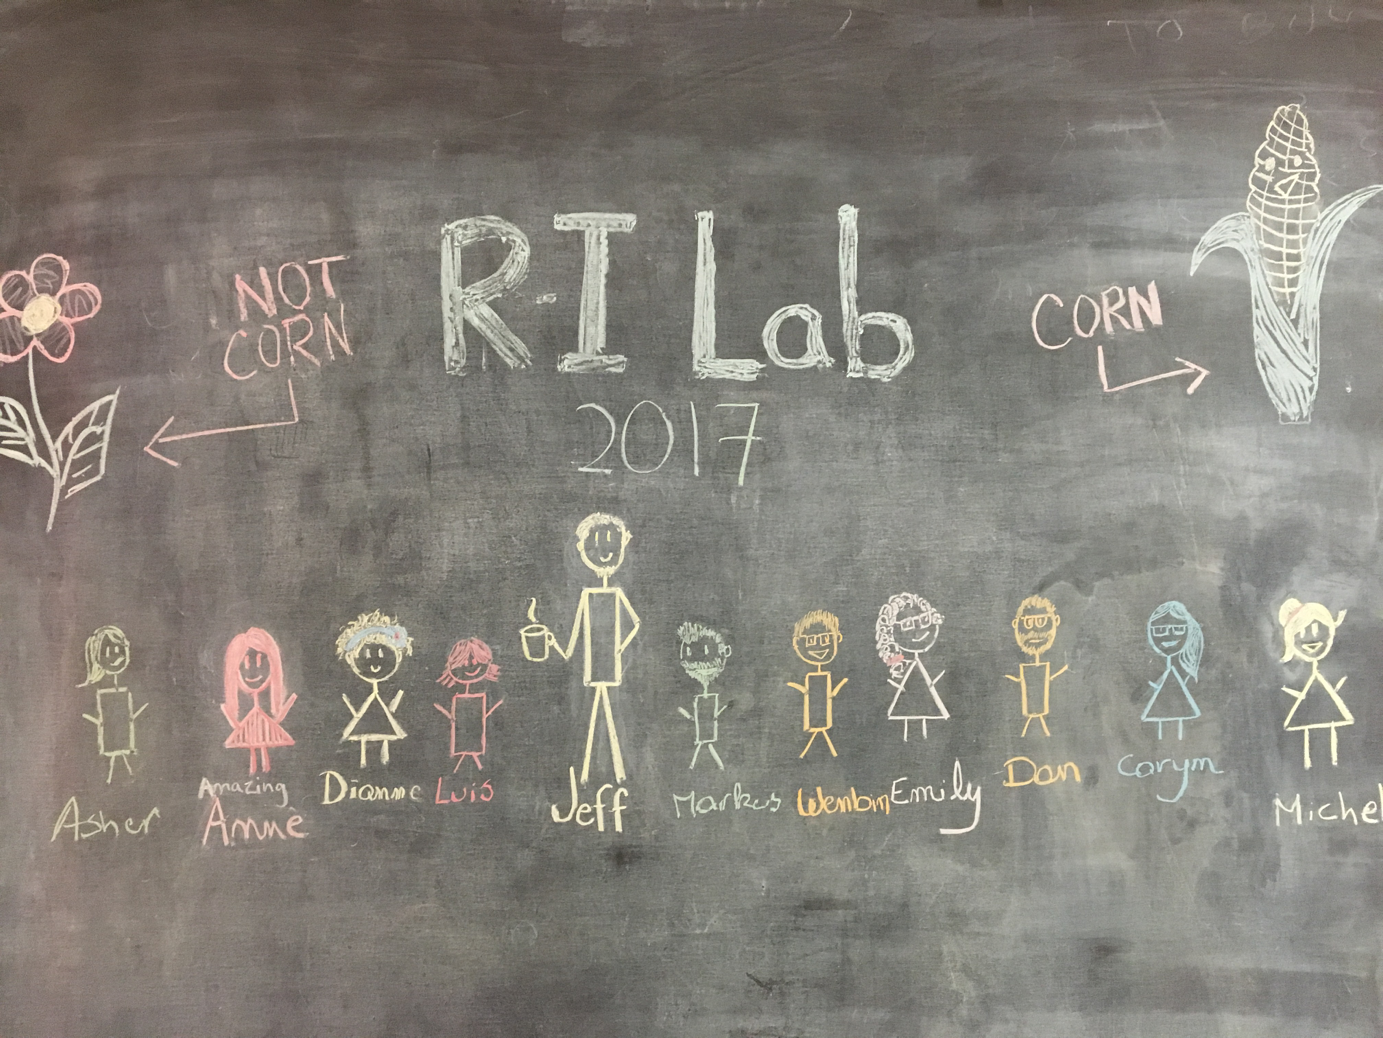
\includegraphics[width=.9\linewidth]{figures/lab_group.png}
\caption{\textbf{Supplemental figure} Test test test}
\label{fig:S1}
\end{figure*}
\pagebreak




\begin{table*}[htbp]
\centering

\caption{\bf Shrink a large table to fit the page}
%\begin{adjustbox}{totalheight=\textheight-2\baselineskip}
\begin{tableminipage}{\textwidth}
\begin{small}
\begin{tabularx}{\textwidth}{sb}
\hline
Parameter & Description \\
\hline
\textbf{Adaptation} & \textbf{Trait related parameters} \\
\hline
Time to optimum & Generations until new optimum is reached \\
Adaptation rate (haldane) & Adaptation rate until new optimum is reached. Calculated as $rate(h) = \frac{\frac{ln(x_2)}{sd_{x_{12}}}-\frac{ln(x_1)}{sd_{x_{12}}}}{t_2-t_1}$ \\
Final genetic variance & Genetic variance in the final generation \\
\textbf{Fixations} & \textbf{Mutations that fix after the optimum shift} \\
\hline
From new mutations (\#) & Sum of fixed mutations in the final population that were already segregating before  the optimum shift \\
From standing variation (\#) & Sum of fixed mutations in the final population that arose after the optimum shift \\
Max. effect size & Maximal effect size of all fixations \\
Mean effect size & Mean effect size of all fixations \\
Mean effect size of negative fixations & Mean effect size of negative mutations \\
Mean effect size of positive fixations & Mean effect size of positive mutations \\
Mean emergence time & Mean generation when a mutation arose that fixed in the last 0.1 N generations \\
Mean fixation time & Mean generation in which a mutation fixed \\
Min. effect size & Minimal effect size of all fixations \\
Negative (\#) & Sum of fixed mutations with negative effects in the final population \\
New/standing fixations & Ratio of mutations from new mutations vs. standing mutations  \\
Proportion negative & Proportion of negative fixations from all mutations \\
Positive (\#) & Sum of fixed mutations with positive effects in the final population \\
SD of effect sizes & Standard deviation of effect sizes of all fixations \\
SD of negative effect sizes & Standard deviation of effect sizes of negative fixations \\
SD of positive effect sizes & Standard deviation of effect sizes of positive fixations \\
Total (\#) & Sum of fixed mutations in the final population \\
\textbf{Sweeps} & \textbf{Mutations that fix faster than 99\% of neutral fixations} \\
\hline
Hard sweeps (\#) & Sum of selective sweeps from new mutations \\
Proportion of hard sweeps & Porportion of hard selective sweeps of all selective sweeps \\
Proportion of sweeps from standing & Proportion of selective sweeps from stainding variation of all selection sweeps \\
Sweeps (\#) & Sum of selective sweeps \\
Sweeps from standing variation (\#) & Sum of selective sweeps from mutations that were already segregating before  the optimum shift \\
Sweeps/fixations & Ratio of sweeps vs. fixations \\
\textbf{Segregating sites} & \textbf{Mutations that segregate in the final generation} \\
\hline
Max. effect size & Maximal effect size of segregating sites \\
Mean effect size & Mean effect size of segregating sites \\
Mean effect size of negative sites & Mean effect size of segregating sites with negative effects \\
Mean effect size of positive sites & Mean effect size of segregating sites with positive effects \\
Mean frequency of all sites & Mean allele frequency of segregating sites \\
Mean frequency of negative sites & Mean allele frequency of segregating sites with negative effects \\
Mean frequency of positive sites & Mean allele frequency of segregating sites with positive effects \\
Min. effect size & Minimal effect size of segregating sites \\
Negative (\#) & Sum of segregating sites with negative effect \\
Positive (\#) & Sum of segregating sites with positive effect \\
Proportion of negative sites & Proportion of segregating sites with negative effect of all segregating sites \\
Standard deviation of effect sizes & Standard deviation of effect sizes of all segregating sites \\
Total (\#) & Sum segregating sites in the final generation \\
\hline

\end{tabularx}
  \label{tab:parameter_list}
  \end{small}
\end{tableminipage}

%\end{adjustbox}
\end{table*}


\end{document}
